\section{Reverse\_Shell}

\begin{center}
    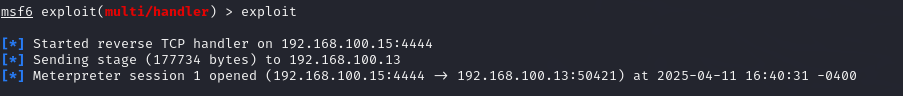
\includegraphics[width=0.8\textwidth]{Question/SC/18_kali.PNG}
\end{center}

\vspace{0.15cm}

\begin{center}
    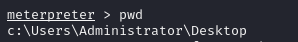
\includegraphics[width=0.6\textwidth]{Question/SC/19_0.PNG}
\end{center}

\vspace{0.15cm}

\begin{center}
    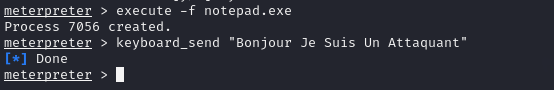
\includegraphics[width=0.6\textwidth]{Question/SC/19.PNG}
\end{center}

\vspace{0.15cm}
\begin{center}
    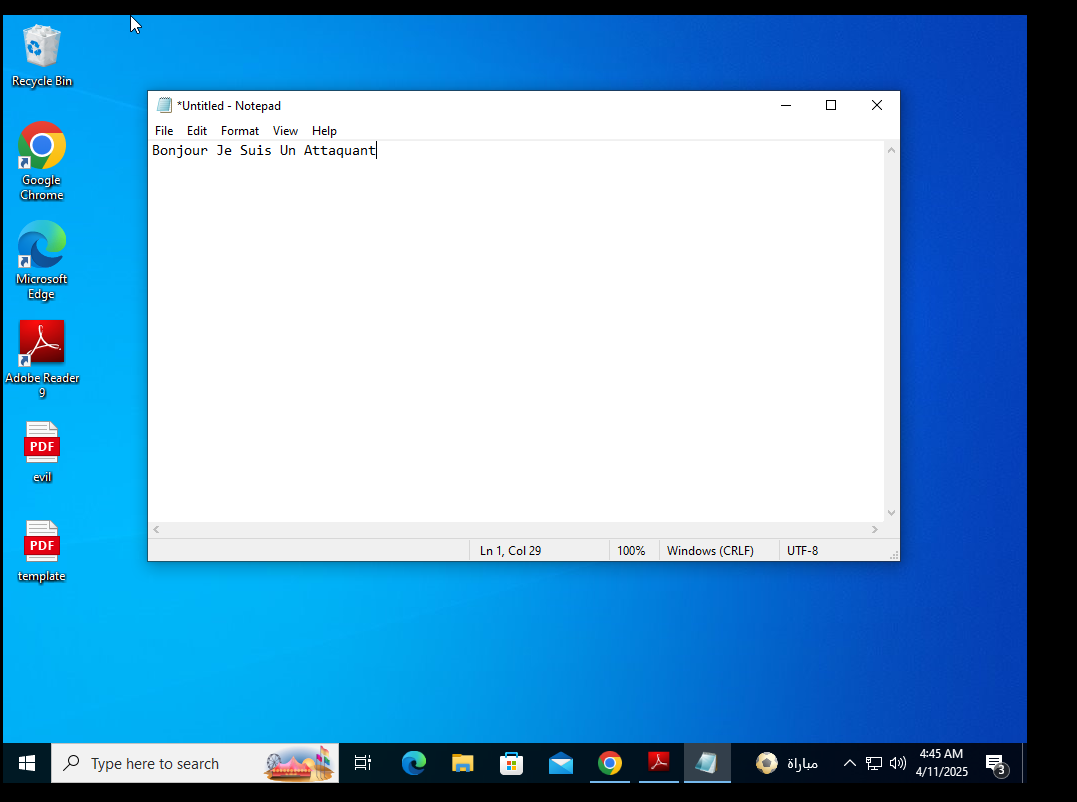
\includegraphics[width=0.6\textwidth]{Question/SC/19_2.PNG}
\end{center}

\vspace{0.15cm}
\begin{center}
    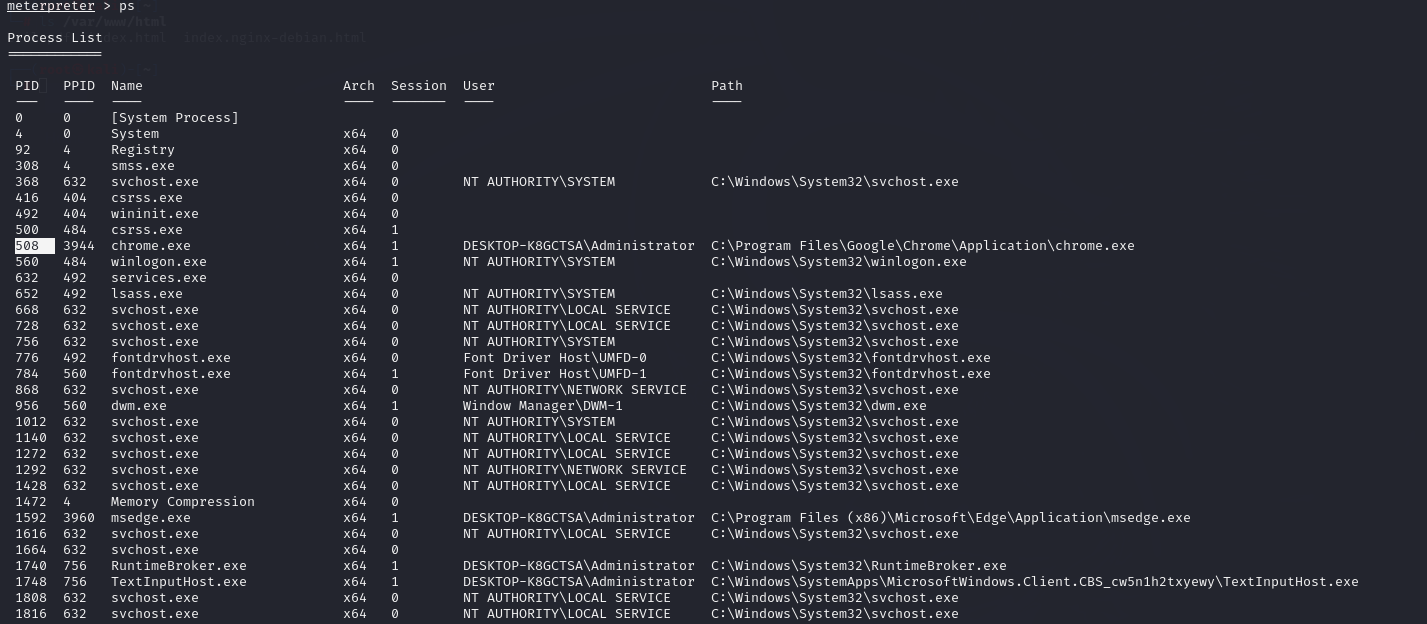
\includegraphics[width=0.6\textwidth]{Question/SC/20_1.PNG}
\end{center}

\vspace{0.15cm}
\begin{center}
    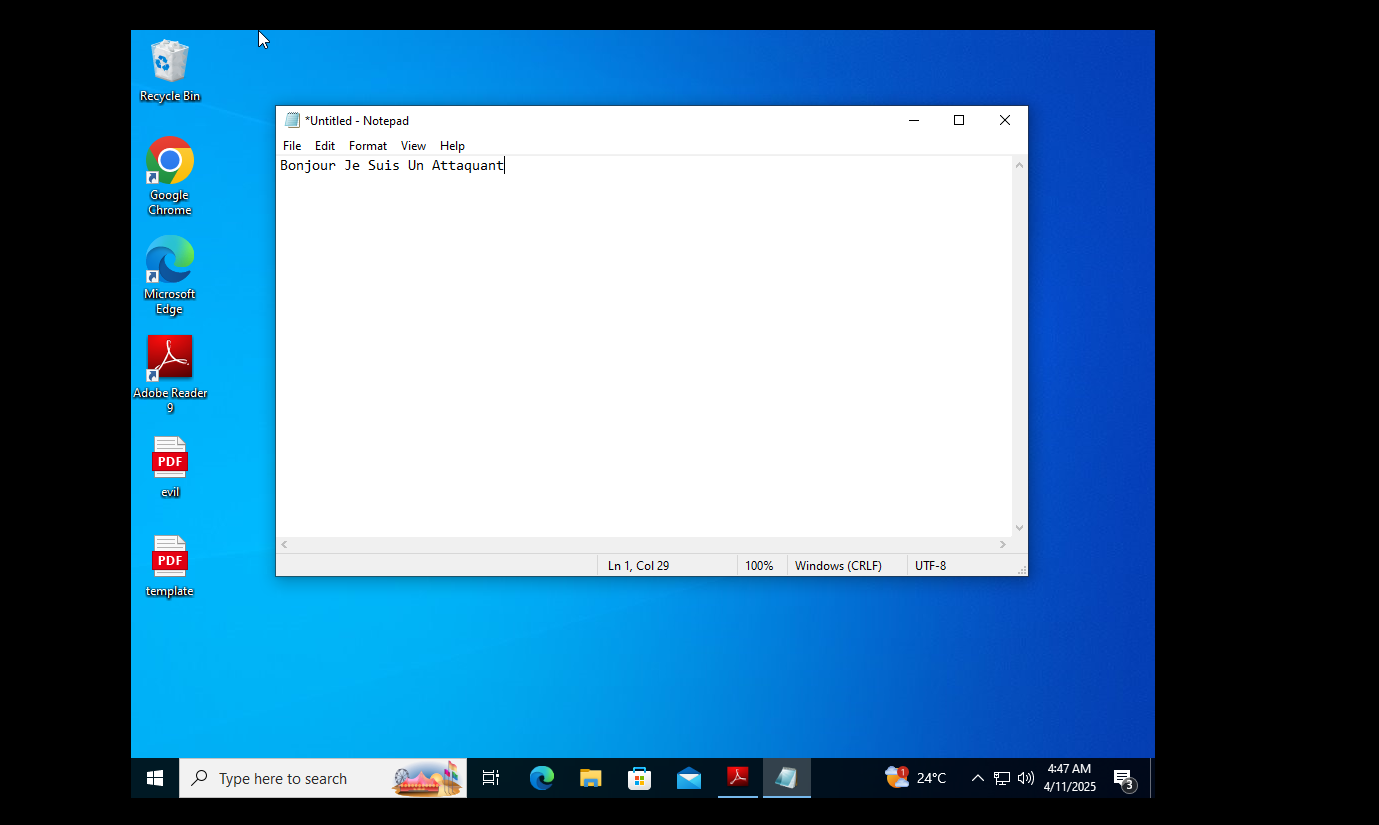
\includegraphics[width=0.6\textwidth]{Question/SC/20_2.PNG}
\end{center}



\vspace{0.35cm}


\begin{prettyBox}{Commandes \& Remarques}{myblue}
    \begin{itemize}
        \item \textbf{Remarque} : Après que l'utilisateur ouvre le fichier \texttt{template.pdf}, le payload s'exécute et l'on peut alors démarrer une session de type \texttt{reverse\_shell}.
        \item \textbf{pwd} : affiche le répertoire courant sur la machine cible.
        \item \textbf{keyboard\_send} : cette commande écrit le message spécifié par l'attaquant directement sur la machine victime. Dans notre cas, le message apparaît dans le bloc-notes (\texttt{notepad.exe}).
        \item \textbf{ps} : affiche les noms, les identifiants (PID), et les chemins d'accès des processus actifs sur la machine cible.
    \end{itemize}
\end{prettyBox}

